% !TeX spellcheck = en_US
\documentclass[a4paper]{article}
\usepackage[a4paper]{geometry}
\usepackage{graphicx}
\usepackage{amsmath}
\usepackage{amssymb}
\usepackage{amsthm}
\usepackage{subcaption}
\usepackage{minted}
\usepackage{mathtools}
\usepackage[ruled,vlined]{algorithm2e}
\usepackage[english]{babel}
\usepackage[hidelinks]{hyperref}

\begin{document}
	\title{Information Theory - AY 2020/2021\\Laboratory Report}
	\author{Amedeo Giuliani - 2005797}
	\date{\today}
	\maketitle
	
	\section{Discrete entropy}
	Given a discrete random variable $ X $, the Shannon entropy is defined as:
	\begin{equation}
		H(X) = -\sum_{x \in A_x} p(x)log_2\ p(x)\quad [bits]
	\end{equation}
	A binary random variable $ X=\{0,1\} $ with $ p(X) = \left(\frac{1}{2},\frac{1}{2}\right) $ has entropy $ H(X)=1\ bit$ and all other distributions yield a lower entropy. To test this, we can generate a sequence X of binary random variables. Then, we count the occurrences of zeros and ones in X and we divide each counter for the sequence length to obtain the empirical probability mass distribution (PMD) $ p(X)=(1-p,p) $, with $ p $ the probability of one. From this, we compute the entropy: $ H(X) = H(p) =1\ bit$, when $ p=\frac{1}{2} $. Instead, for example, $ p = 0.3 $ yields $ H(x)=1\ bit $.
	\subsection{Joint entropy}
	The joint entropy of a pair of discrete random variables $ X,Y $ is defined as:
	\begin{equation}
		H(X,Y) = -\sum_{x \in A_x}\sum_{y\in A_y} p(x,y)log_2\ p(x,y) = H(X)+H(Y|X)
	\end{equation}
	If we consider another random variable $ Z=\{0,1\} $ with $ p(Z)\equiv p(X) $, independent from $ X $, their joint entropy will be
	\begin{equation}
		H(X,Z) = H(X)+H(Z|X) = H(X)+H(Z) = 2\ bits
	\end{equation}
	Instead, if we consider $ Y=1-X $, the joint entropy between $ X $ and $ Y $ will be
	\begin{equation}
		H(X,Y) = H(X) = 1\ bit
	\end{equation}
	as $ Y $ is a function of $ X $. In fact, if we run another simulation, we find out that $ H(Z)=1 bit $, $ H(X,Y) = 1\ bit $ and $ H(X,Z) = 1.99\ bits $, which confirms the theory results.\\
	To compute the joint distribution and the joint entropy, the following Python functions has been employed:
	\begin{minted}{Python}
def getJointEntropy(joint_pdf):
	return -sum(np.multiply(joint_pdf[joint_pdf!=0],\
	np.log2(joint_pdf[joint_pdf!=0])))
		
def getJointDistribution(s1,s2,b):
	h,_,_ = np.histogram2d(s1,s2,bins=b)
	joint_pdf = h.flatten()/len(s1)
	return joint_pdf
	\end{minted}
	\subsection{Kullback-Leiber Divergence}
	The KLD, or relative entropy, between two PMDs is defined as:
	\begin{equation}
		D(p||q) = \sum_{x \in A_x}p(x)log_2\frac{p(x)}{q(x)}
	\end{equation}
	It measures ``the distance'' between the two PMDs, thus it is zero when $ p\equiv q$. In fact, considering the previous scenario, $ D(p_x||p_y)=0.02\ bits$ and $ D(p_x||p_z) = 0.01\ bits$, i.e., almost zero, since $ X $, $ Y $ and $ Z $ have all the same distributions.  
	\subsection{Mutual Information}
	The mutual information between two discrete random variables $ X,Y $ is defined as:
	\begin{equation}
		\sum_{x \in A_x} \sum_{y\in A_y} p(x,y)log_2\frac{p(x,y)}{p(x)p(y)} = D(p(x,y)||p(x)p(y))
	\end{equation}
	But it can also be expressed in the following equivalent ways:
	\begin{align}
		I(X;Y) &= H(X)-H(X|Y) \\
		I(X;Y) &= H(Y)-H(Y|X) \\
		I(X;Y) &= H(X)+H(Y)-H(X,Y)
	\end{align}
	Hence, if the two random variables are independent, their mutual information is zero. Again, by resuming the previous experiment, we find that $ I(X;Z) = 0.01\ bits $, i.e., almost zero, as they are independent, and that $ I(X;Y) = 1\ bit = H(X)$ as $ Y $ is a function of $ X $.
	\section{Data Processing Inequality}
	The Data Processing Inequality (DPI) states that, if $ X,Y,Z $ are in a Markov relation (in that order), i.e., $ X \xleftrightarrow{} Y \xleftrightarrow{} Z $, then
	\begin{equation}
		I(X;Y) \ge I(X;Z)
	\end{equation}
	Consider a scenario in which a discrete random variable $ X $, generated according to a certain distribution $ p(X) $, is the input of a Binary Simmetric Channel (BSC) and, in turn, the output $ Y $ is the input of another BSC. Hence, Z is the overall output of this cascade of BSCs, as in Fig.~\ref{fig:bsc_cascade}. Here $ X,Y,Z $ are in a Markov relation in that order. By estimating the mutual information between $ X $ and $ Y $ and between $ X $ and $ Z $, we find that $ I(X;Y) = 0.1\ bits $ and $ I(X;Z) = 0.07\ bits $. If we perform a more in-depth analysis, by repeating the experiment independently for K times, we find that $ I(X;Y) \ge I(X;Z) $ always, as in Fig.~\ref{fig:mi_bsc_cascade}. We have indeed verified that the DPI holds every time $ X \xleftrightarrow{} Y \xleftrightarrow{} Z $.
	\begin{figure}[!h]
		\centering
		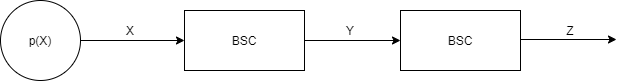
\includegraphics[width=0.7\linewidth]{bsc_cascade.png}
		\caption{Cascade of two BSCs.}
		\label{fig:bsc_cascade}
	\end{figure}
	\begin{figure}[!h]
		\centering
		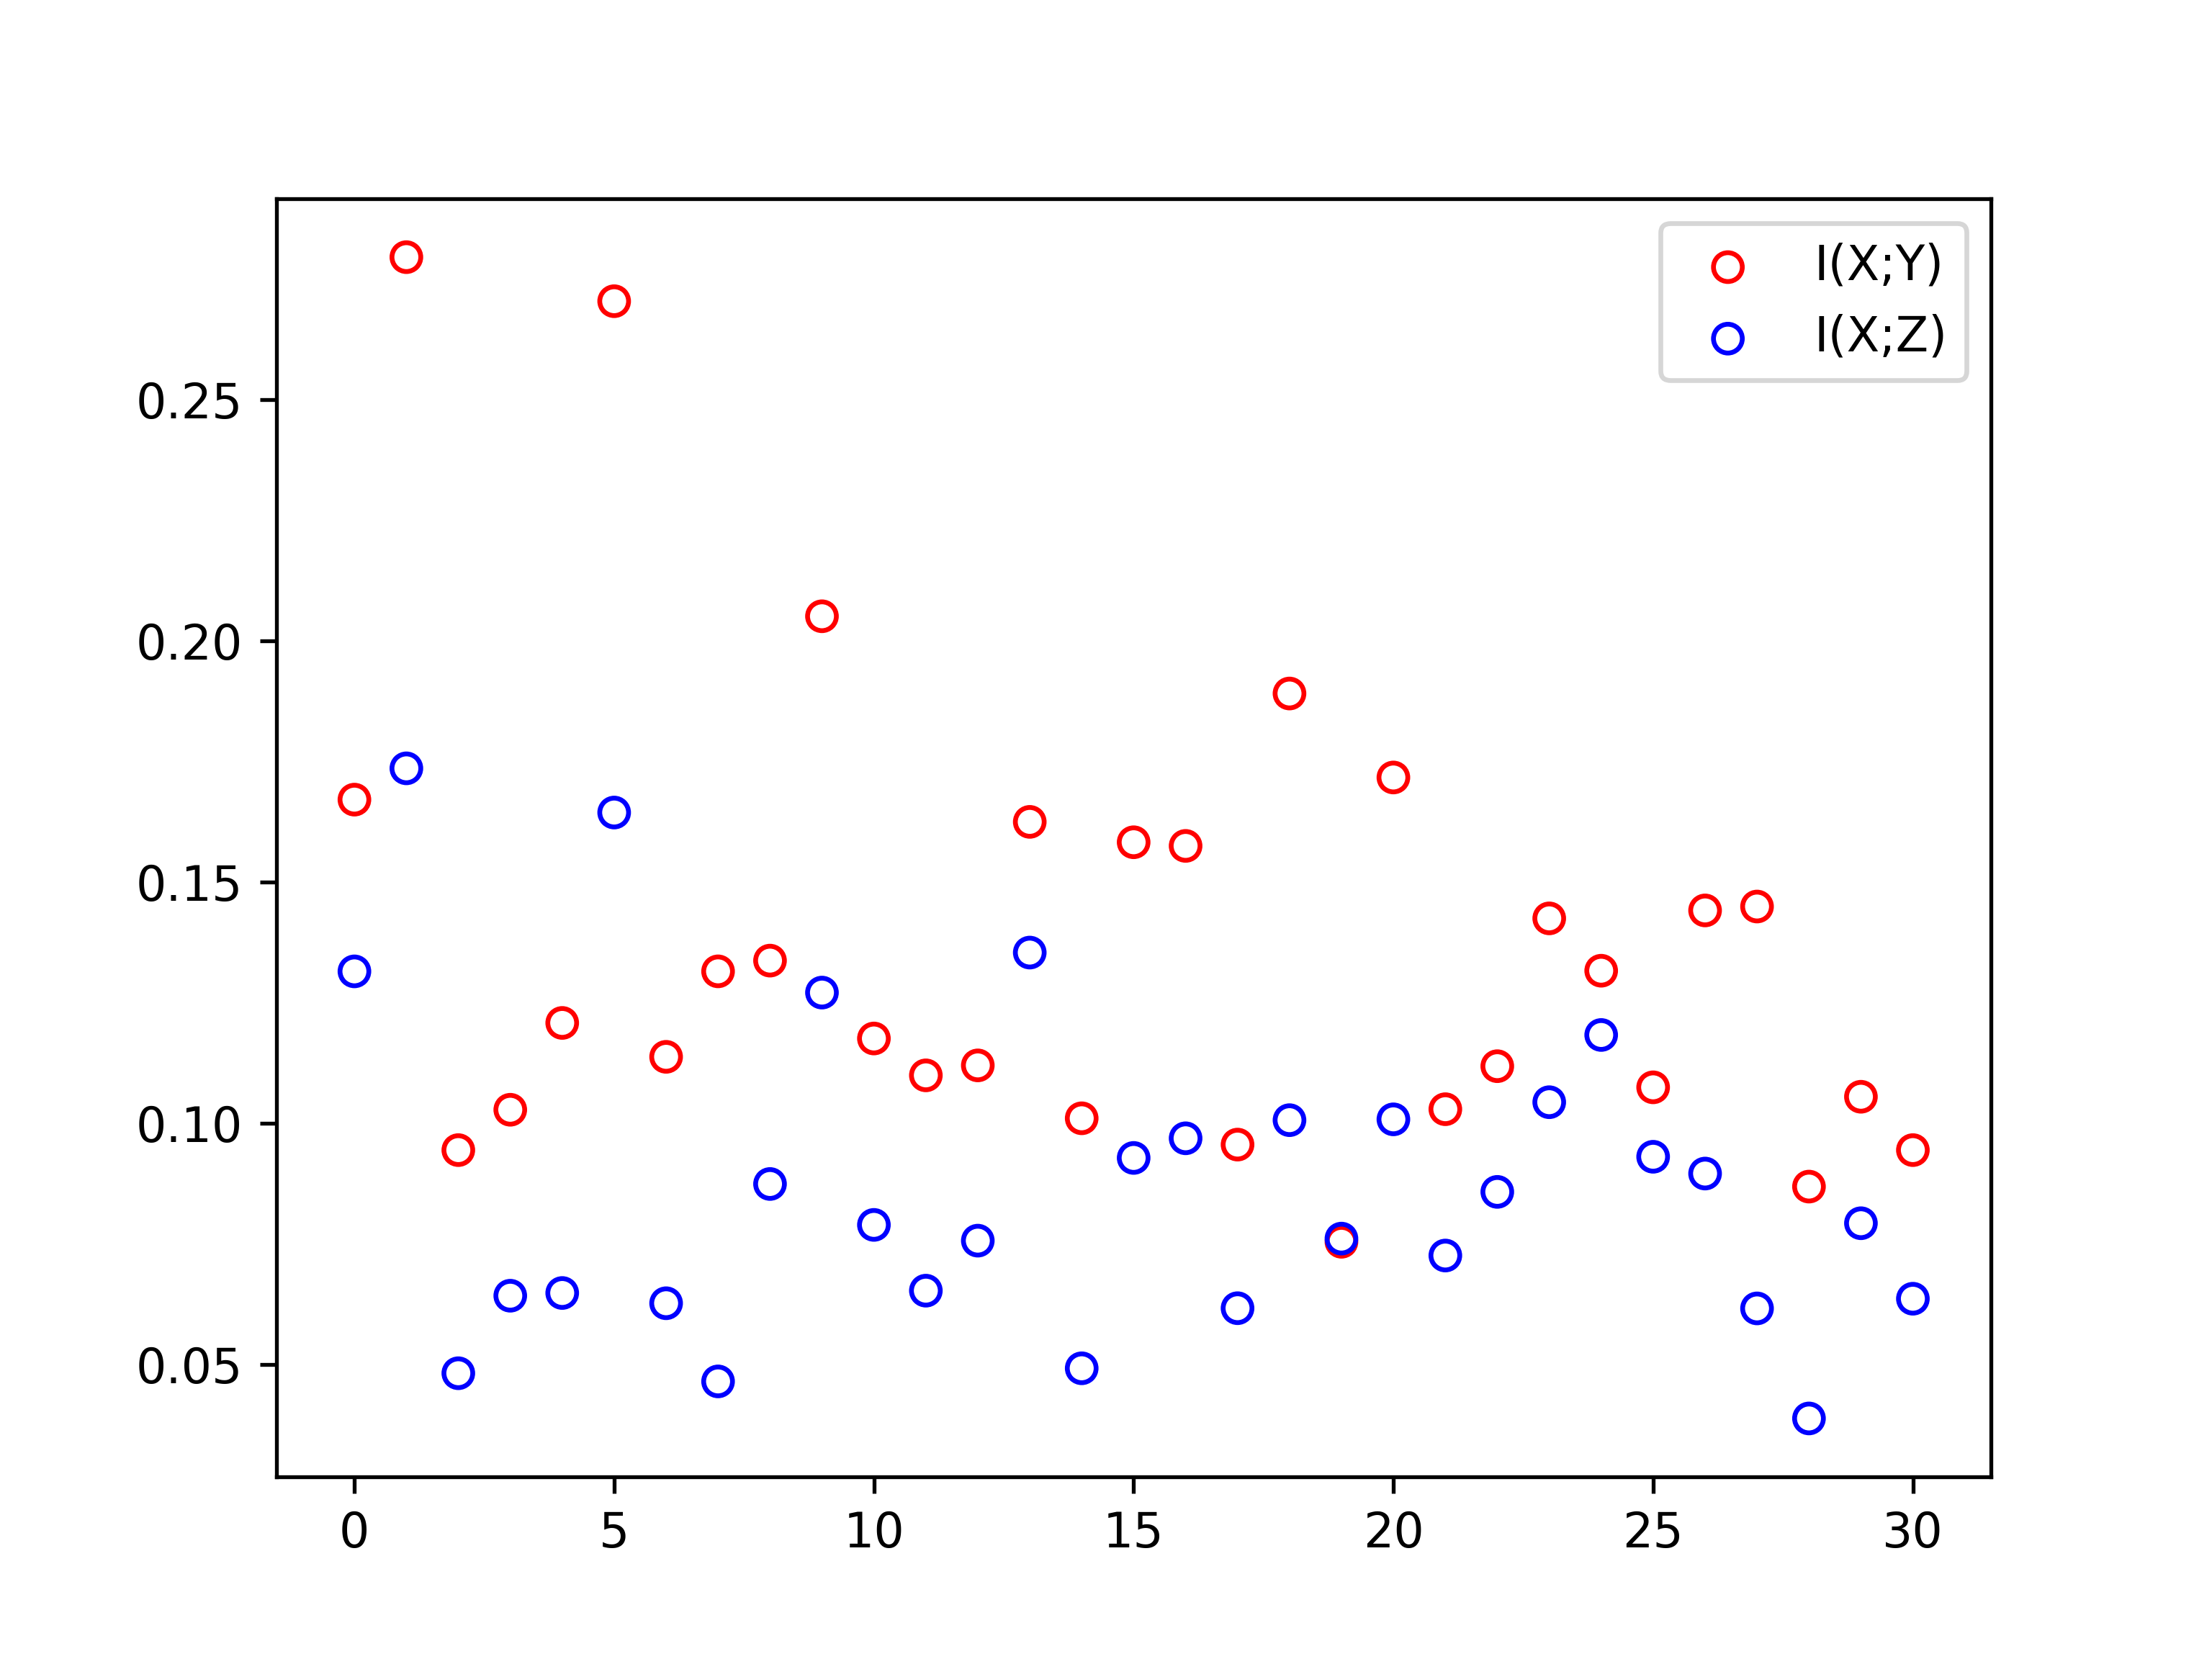
\includegraphics[width=0.7\linewidth]{mi.png}
		\caption{}
		\label{fig:mi_bsc_cascade}
	\end{figure}
	\section{Asymptotic Equipartition Property}
	The Asymptotic Equipartition Property (AEP) states that, considering a word $ \boldsymbol{x} $ made of n symbols, for any $\epsilon > 0$
	\begin{equation}
		\lim_{n\rightarrow+\infty} \mathbb{P}[\boldsymbol{x}\in \mathcal{T}_x(\epsilon,n)] = 1
	\end{equation}
	This means that the probability of $ \boldsymbol{x} $ being a weakly $\epsilon$-typical sequence for a message $ \{x_\ell\} $ with i.i.d. symbols tends to one as n grows to infinity.
	To verify this property, we set up a Monte-Carlo simulation with parameters:
	\begin{itemize}
		\item n, sequence length
		\item q, probability of zero (thus p = 1-q is the probability of one)
		\item $\epsilon$, the $\epsilon$-typicality parameter
		\item K, number of trials to estimate the probability
	\end{itemize}
	The implemented algorithm is summarized in Algo.~\ref{algo:aep}. As expected, with growing n, the probability ``prob'' approaches one, as depicted in Fig.~\ref{fig:aep}. In particular, with n = 5, $ \mathbb{P}[\boldsymbol{x}\in \mathcal{T}_x(\epsilon,n)] = 39.27\% $, while with n = 200 we have $ \mathbb{P}[\boldsymbol{x}\in \mathcal{T}_x(\epsilon,n)] = 99.75\% $.
	\begin{figure}
		\centering
		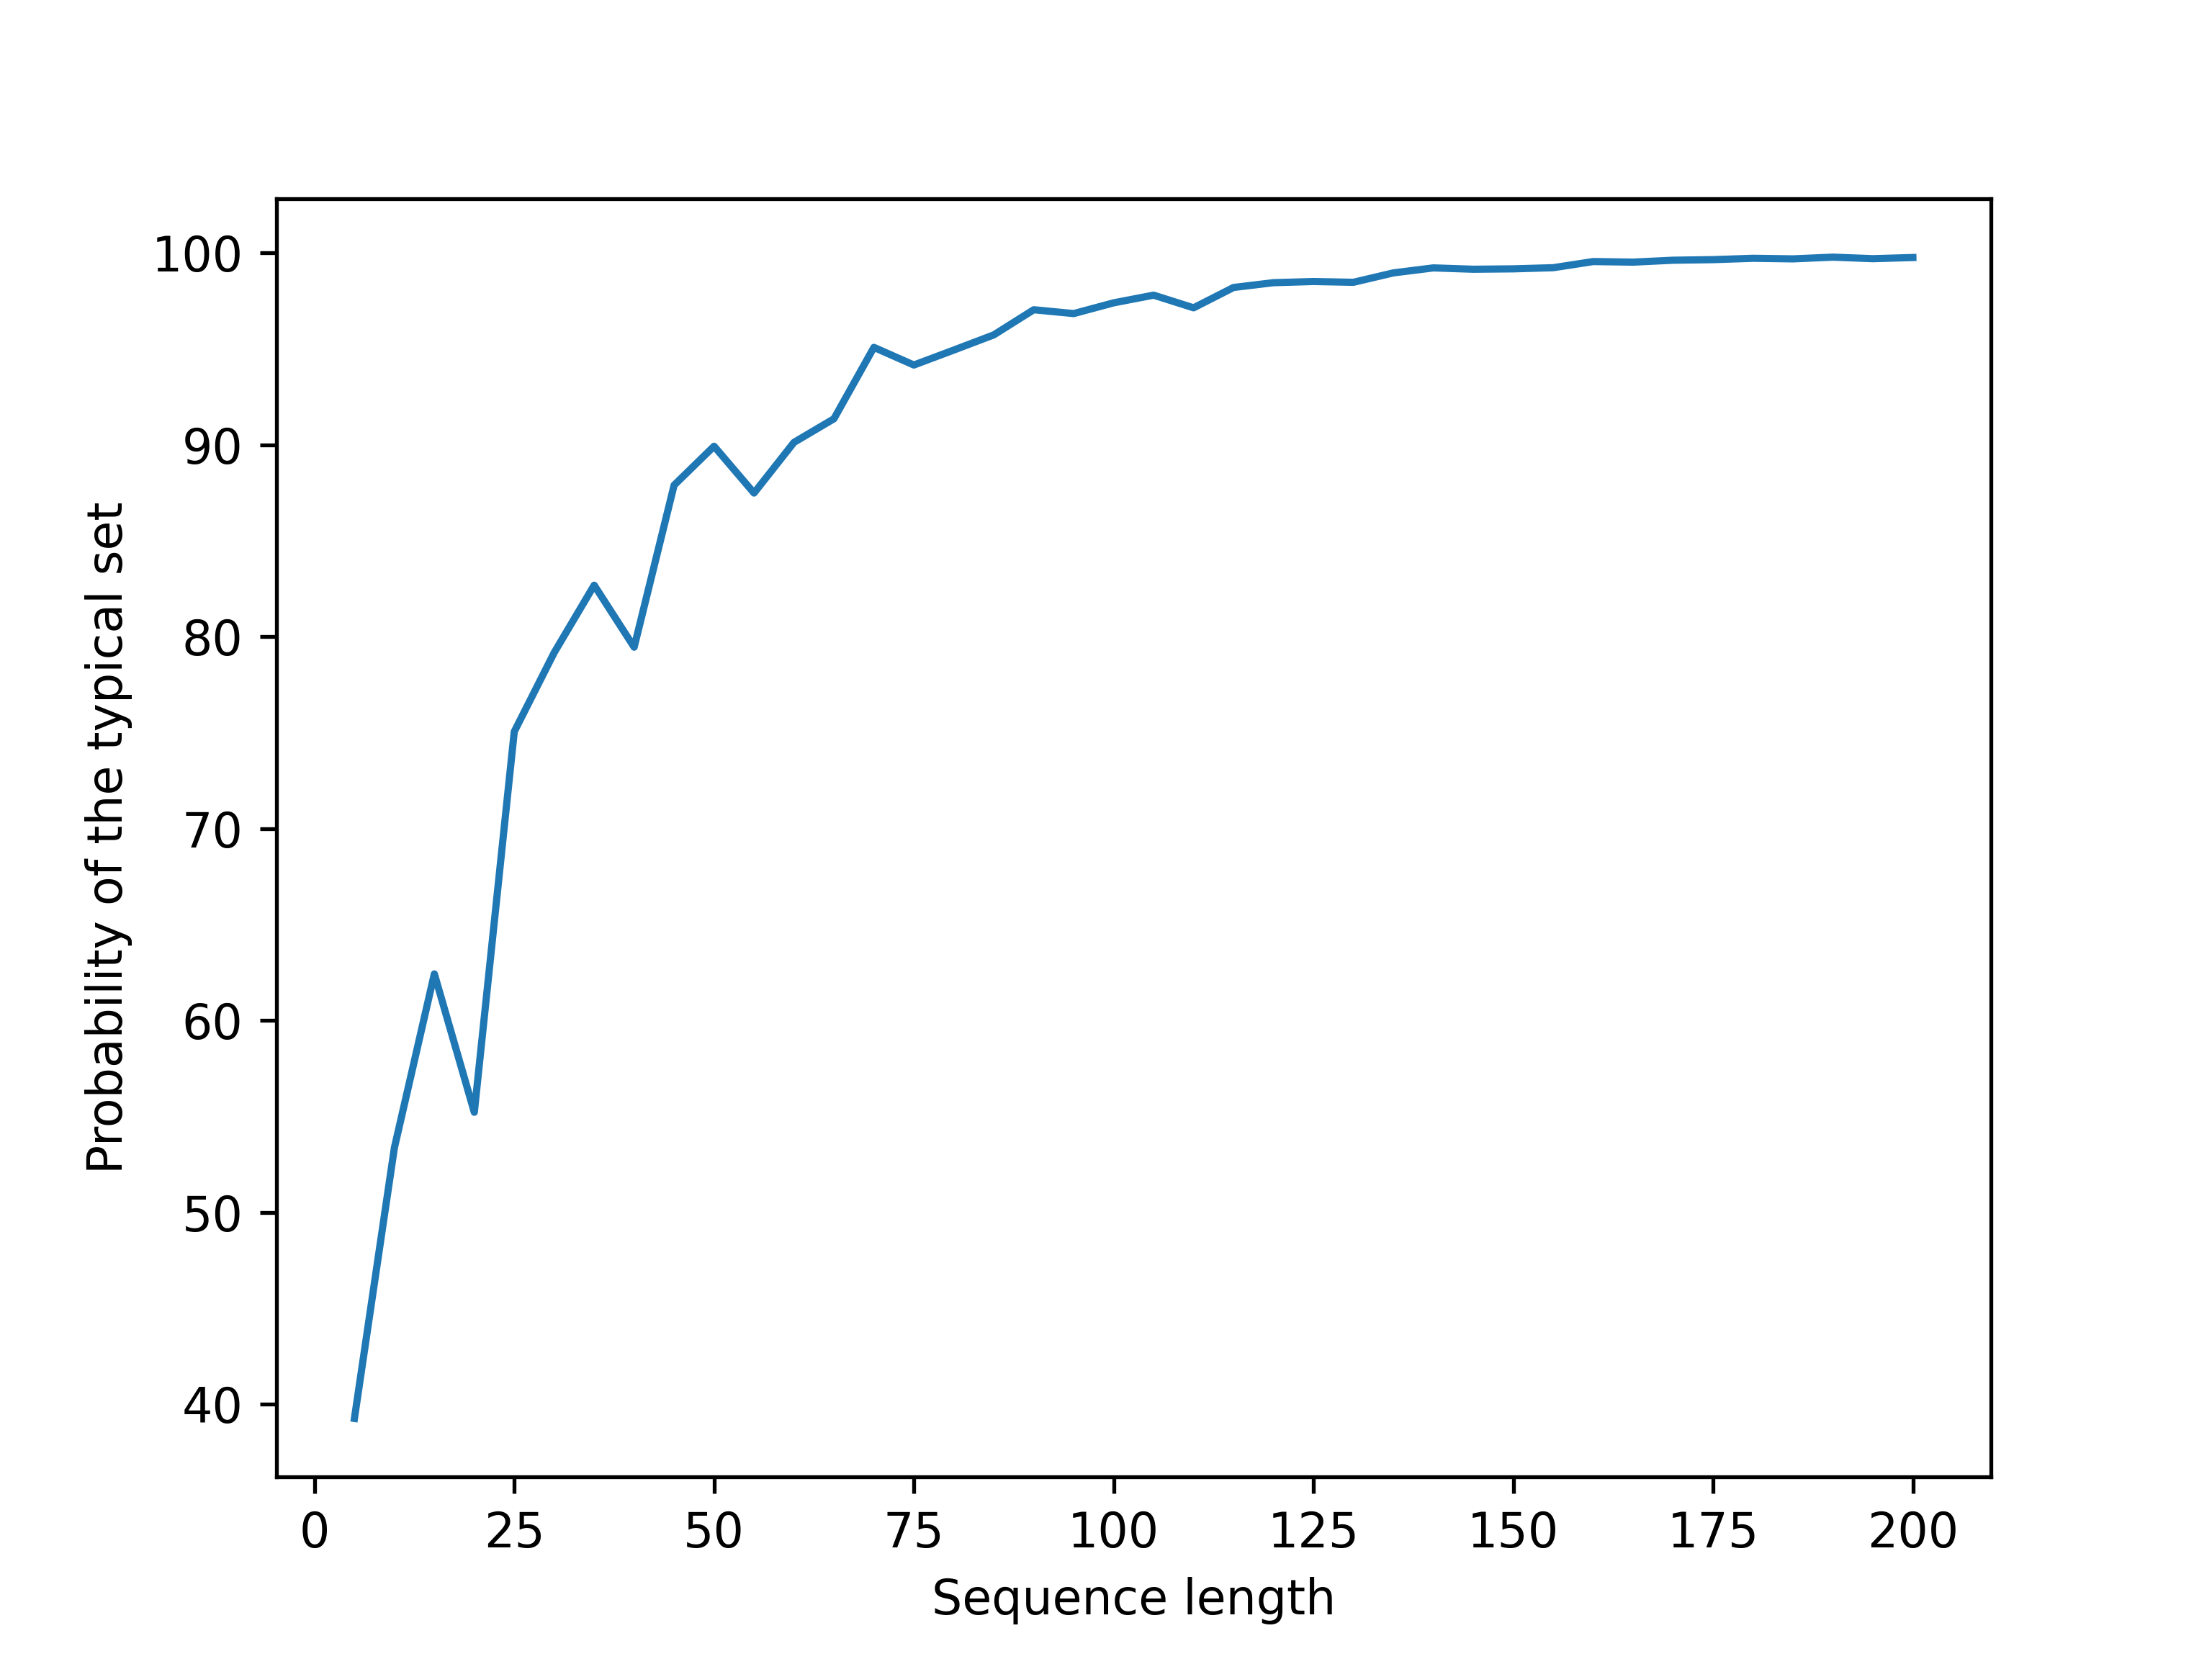
\includegraphics[width=0.7\linewidth]{aep.png}
		\caption{}
		\label{fig:aep}
	\end{figure}
	\begin{algorithm}
		\SetAlgoLined
		\caption{AEP test}
		set n = 5, N = 200, K = 1e4, q = 0.25 and $\epsilon$=0.15\;
		compute the entropy H(q)\;
		lowerBound = H(q)-$\epsilon$\;
		upperBound = H(q)+$\epsilon$\;
		\While{n $\le$ N}{
			count = 0\;
			\For{k=0 ; k$ < $K ; k++}{
				generate sequence of zeros and ones long n\;
				count zeros in sequence\;
				count ones in sequence\;
				compute average information per symbol\;
				\If{average information per symbol is within the bounds}{
					count++\;
				}
			}
			prob = count/K\;
			n = n + 5\;
		}
	\label{algo:aep}
	\end{algorithm}
	\newpage
	\section{AWGN channel capacity}
	The capacity of a discrete-time AWGN channel with gain $ g=1 $, symbol time $ T=1 $, i.i.d. noise $ z_n \sim \mathcal{N}(0,\sigma_z^2) $ and input power constraint $ \mathbb{E}[x_n^2] \le P $ is achieved with memory-less input $ x_n \sim \mathcal{N}(0,P)$ and it is:
	\begin{equation}
		C_{awgn} = \frac{1}{2} log_2 \left( 1 + \frac{P}{\sigma_z^2} \right)
	\end{equation}
	To test this theorem, we can set up a simulation in which we generate a sequence $ x $ of n i.i.d. Gaussian symbols with mean $ m_x = 0 $ and standard deviation $ \sigma_x = 1 $. Then, we analyze what we receive at the output of the AWGN channel. From theory, we know that the output is Gaussian as well, with same mean and $ \sigma_y^2 = P + \sigma_z^2 $. Hence, we perform a Gaussian distribution fitting to estimate the parameters of the output distribution. From here, the derivation of the actual information rate is straightforward: $ R = \frac{1}{2} log_2 \left( \frac{\sigma_y^2}{\sigma_z^2} \right) $.\\
	We can repeat the experiment independently K times to compare the actual data rate and the capacity.
	From Fig.~\ref{fig:awgncap} we can clearly see that, on average, the actual rate R is equal to the capacity C.
	\begin{figure}[!h]
		\centering
		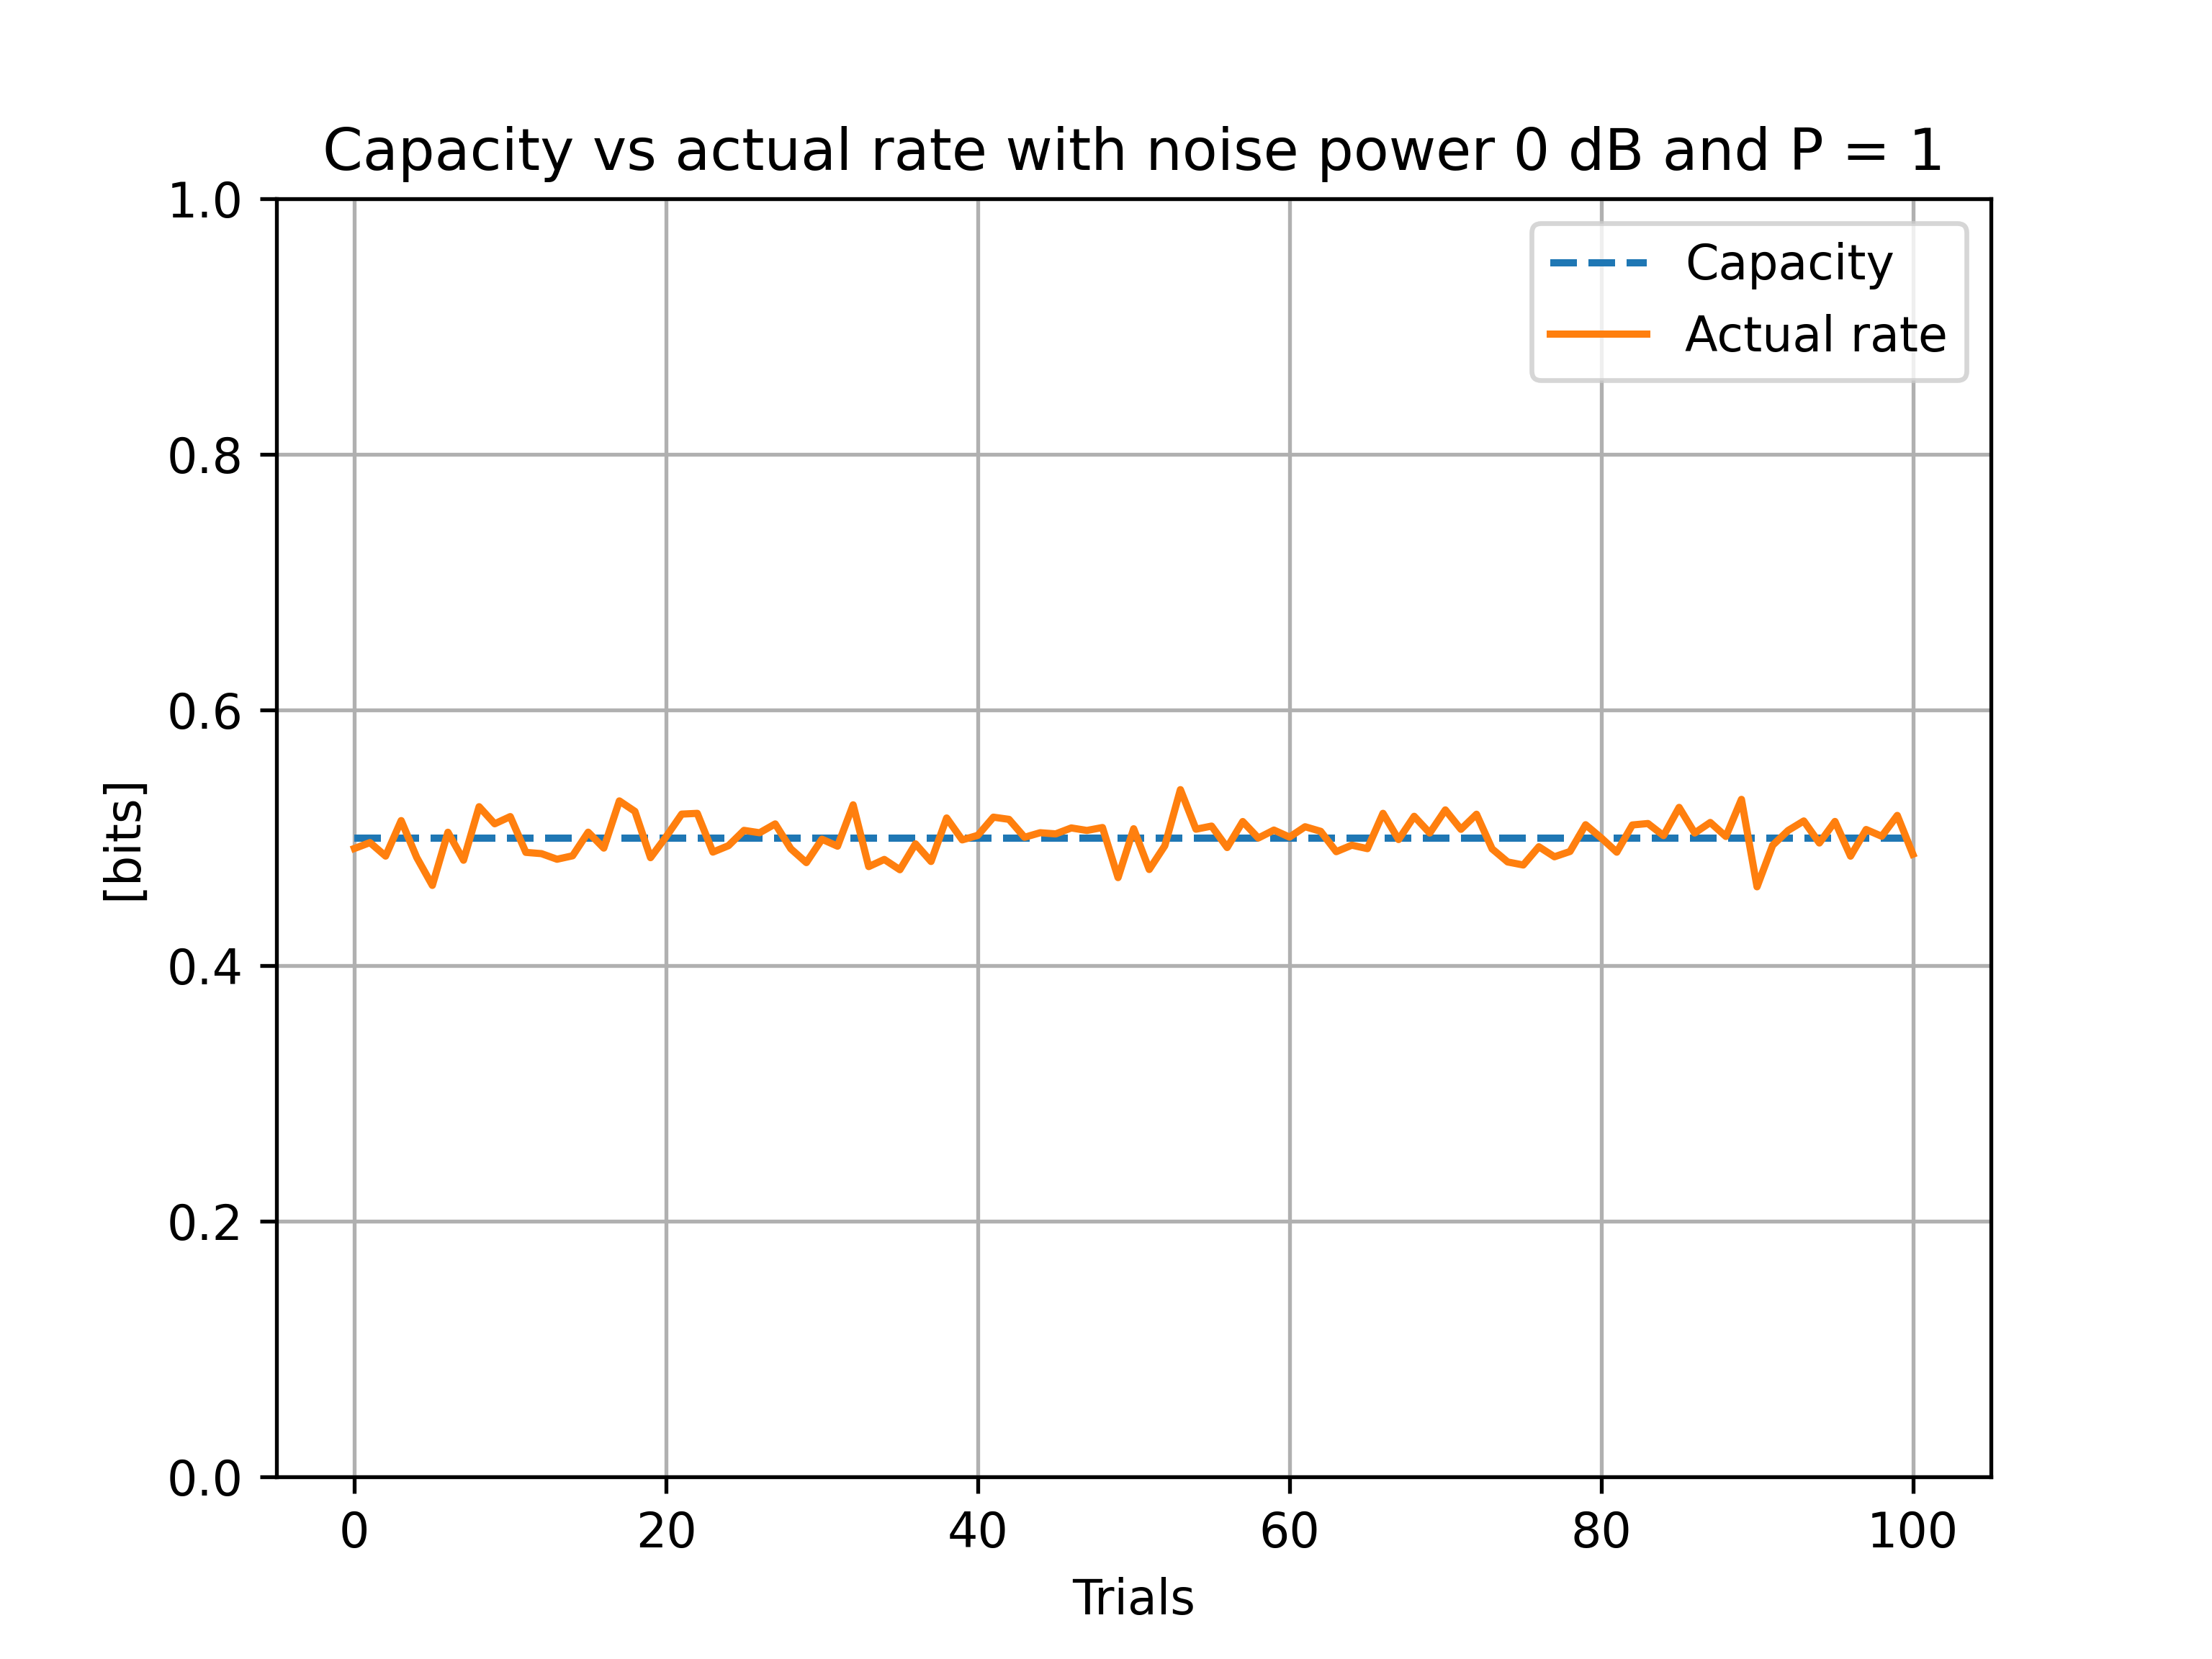
\includegraphics[width=0.7\linewidth]{cap.png}
		\caption{}
		\label{fig:awgncap}
	\end{figure}
\end{document}